\section{编码模型}
\label{sec:lossless-model}

“用较少的0和1记录消息”要变成数学问题，得先说清四件事：消息从哪里来，编码把什么映射成什么，解码要恢复什么，以及“较少”按什么标准计算。本节依次固定这些约定，并引入贯穿全章的四符号例子。

\paragraph{信源与消息}
设$\mathcal{X}$是有限集合，称为\term{字母表}（alphabet）。\term{信源}（source）是取值于$\mathcal{X}$的随机变量$X$，其概率质量函数记作
\[
 p(x)=\mathbb{P}(X=x),\qquad x\in\mathcal{X}.
\]
信源连续发出$n$个符号时，得到长度为$n$的消息$X_{1:n}=(X_1,\dots,X_n)$，它的取值记作$x_{1:n}$。本章除非特别说明，都假设$X_1,X_2,\dots$独立同分布，每个都服从$p$，于是
\begin{equation}
 \mathbb{P}(X_{1:n}=x_{1:n})=p(x_{1:n})=\prod_{i=1}^{n}p(x_i).
 \label{eq:lossless-product}
\end{equation}
这里$p(x_{1:n})$是长度为$n$的消息的概率，用同一个字母$p$记，参数的形状说明它指哪一个。

概率为零的符号永远不会出现，对平均量也没有贡献。本章约定把它们从字母表中去掉，即$p(x)>0$对每个$x\in\mathcal{X}$成立；需要讨论“设计时以为某个符号不会出现”的情形时（第~\ref{sec:lossless-arithmetic}小节和第~\ref{sec:lossless-finite-resources}节），再单独说明。

\paragraph{码字与编码}
记$\{0,1\}^{*}$为所有有限长二进制串的集合，其中包括长度为零的空串。二进制串$s$的长度记作$\lvert s\rvert$。一个\term{二进制码}（binary code）是映射
\[
 c:\mathcal{X}\to\{0,1\}^{*},
\]
$c(x)$称为符号$x$的\term{码字}（codeword），$\ell(x)=\lvert c(x)\rvert$称为它的码长。逐符号编码一条消息时，把各符号的码字依次拼接起来，
\begin{equation}
 c(x_{1:n})=c(x_1)c(x_2)\cdots c(x_n),
 \label{eq:lossless-extension}
\end{equation}
这个映射称为\term{码的扩展}（extension of a code）。\term{编码器}（encoder）执行这一映射，\term{解码器}（decoder）从收到的二进制串恢复消息。

\paragraph{贯穿全章的例子}
取$\mathcal{X}=\{a,b,c,d\}$，概率表为
\[
 p(a)=0.4,\quad p(b)=0.3,\quad p(c)=0.2,\quad p(d)=0.1 .
\]
码表取$a\mapsto0$、$b\mapsto10$、$c\mapsto110$、$d\mapsto111$。消息$abac$编码成
\[
 c(abac)=0\;10\;0\;110=0100110,
\]
共$7$位，比每符号两位的定长码少$1$位。解码器从左往右读：读到$0$就是$a$；读到$10$就是$b$；再读到$0$是$a$；最后$110$是$c$。图~\ref{fig:lossless-coding-model}画出这一过程。为什么这张码表能这样一步步读出来，是第~\ref{sec:lossless-decodability}节的问题。

\begin{BookInlineFigure}
 \centering
 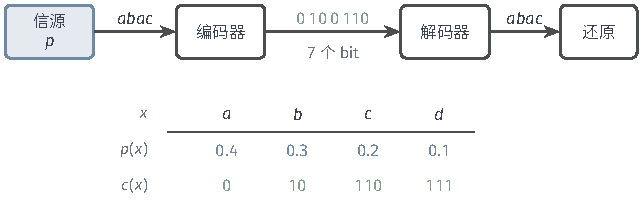
\includegraphics[width=108mm]{figures/07-probability/05-source-coding/tikz/lossless-coding-model/figure.pdf}
 \caption{无损编码的模型。信源（蓝框）按概率表$p$发出消息$abac$，编码器按下方码表把每个符号换成码字并依次拼接（绿色），得到$7$位二进制串；解码器从二进制串精确恢复出同一条消息。}
 \label{fig:lossless-coding-model}
\end{BookInlineFigure}

\paragraph{逐符号与整块，变长与定长}
上面的码表一次处理一个符号，称为逐符号编码。也可以先把$n$个符号组成一块，把整块$x_{1:n}$看成字母表$\mathcal{X}^n$中的一个“大符号”，直接给它分配码字，这就是\term{块编码}（block coding）。整块编码时，被编码的字母表从$\lvert\mathcal{X}\rvert$个元素变成$\lvert\mathcal{X}\rvert^n$个元素，码表的规模随之增长。

码字长度也有两种安排。所有码字等长的称为\term{定长码}（fixed-length code），例如每符号两位的码，或者给每个长度为$n$的块分配同样多位的码；码字长度可以不同的称为\term{变长码}（variable-length code）。定长码不需要寻找码字边界，按固定位数切开即可；变长码要靠码表本身的结构来确定边界。

\paragraph{解码恢复什么}
无损编码要求精确还原，但“还原什么”需要约定。逐符号编码时，解码器要从拼接串$c(x_{1:n})$恢复整条符号序列$x_{1:n}$，而不仅是某一个符号。整块编码时，解码器恢复的是块$x_{1:n}$本身。另一个必须事先约定的是消息长度：解码器是否事先知道$n$，还是要从二进制串本身判断消息在哪里结束。这两种约定的差别在第~\ref{sec:lossless-average-length}节处理确定源时、在第~\ref{sec:lossless-arithmetic}小节处理算术编码的终止时都会出现。

\paragraph{三个评价量}
衡量一个编码方案时，本章分别使用三个量。第一个是按信源概率加权的\term{平均码长}（expected code length），
\begin{equation}
 L(c)=\mathbb{E}[\ell(X)]=\sum_{x\in\mathcal{X}}p(x)\ell(x),
 \label{eq:lossless-average-length}
\end{equation}
它回答长期平均每个符号用多少位：由第~\ref{chap:laws-of-large-numbers}章的大数律，独立编码$n$个符号的总位数除以$n$趋于$L(c)$。第二个是最坏码长$\max_{x}\ell(x)$，它决定缓冲区要准备多大、单条消息最多会多长。第三个是还原错误概率，即解码结果与原消息不同的概率。

三个量回答不同的问题。例中变长码的平均码长是
\[
 L(c)=0.4\times1+0.3\times2+0.2\times3+0.1\times3=1.9 ,
\]
比定长码的$2$少；但最坏码长是$3$，比定长码的$2$多。消息$ddd$用变长码要$9$位，用定长码只要$6$位。所以变长码的“节省”只是平均意义上的，第~\ref{sec:lossless-decodability}节至第~\ref{sec:lossless-methods}节都要求错误概率为零、以平均码长为主要指标，第~\ref{sec:lossless-block-limits}节再允许错误概率为正但趋于零，换取定长的码字。
